\section{Procedimento Strutturato}\label{sec:structuredprocess}
Prima di poter procedere è necessario decidere come realizzare il {\bf procedimento strutturato}.
Esso dovrà poi anche venir modificato dalle {\it variazioni} e dai {\it suggerimenti} dei clienti.

Il modo più {\it flessibile} di rappresentare un procedimento di preparazione di un piatto
in fasi è quello di una struttura a {\it branches} --- ossia rappresentare il procedimento
di preparazione di una ricetta tramite una struttura come la seguente:

\vspace{5pt}\centerline{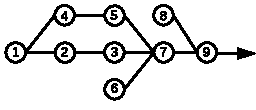
\includegraphics[width=0.8\textwidth]{ex-struct-process-1}}

\vspace{15pt}

Dove ogni {\it nodo numerato} rappresenta una {\it fase}. Ogni fase (nodo) ha zero o più fasi
che la {\it precedono} e zero o più fasi che la {\it seguono}. L'unica regola da imporre
è che ci sia {\it una ed una sola} fase ($F_{9}$) che non ha alcuna fase successiva (una sola
foglia). Altrimenti si verebbe a produrre più di un piatto (che è assurdo).

Con una struttura del genere è possibile ad esempio imporre che per iniziare una fase,
tutte le fasi precedenti ad essa devono essere portate a termine. Ad esempio nella struttura precedente:
$F_{5}$ può essere iniziata solo dopo che $F_{4}$ (e di conseguenza anche $F_{1}$) è stata completata.
$F_{7}$ può essere iniziata solo dopo che $F_{3}$ (e di conseguenza anche $F_{2}$ e $F_{1}$),
$F_{5}$ (e di conseguenza anche $F_{4}$) e $F_{6}$ sono state completate.

Possiamo inoltre {\it parallelizzare} la produzione del piatto. Ad esempio $F_{4}$ e $F_{5}$ possono essere
svolte da un cuoco mentre un altro cuoco sta svolgendo $F_{2}$ e $F_{3}$ (l'importante è che
$F_{1}$ sia stata portata a termine prima di iniziare $F_{2}$ e $F_{4}$). Nel mentre un altro
cuoco ancora può svolgere $F_{6}$ (in questo caso $F_{6}$ può iniziare anche prima di $F_{1}$)
e un altro ancora può svolgere $F_{8}$.

Per poter realizzare una struttura come questa in un database relazionale, sarà necessario
introdurre una {\it relazione ricorsiva}: l'entità che rappresenterà una fase dovrà essere
messa in una {\it relazione molti-a-molti} con se stessa. Infatti ogni fase deve essere
messa in relazione con le sue fasi precedenti (nell'immagine precedente: ogni collegamento
tra due fasi è una relazione).
La relazione ({\tt Precedente}) che permette la realizzazione di tale struttura è mostrata
nel {\it diagramma entità-relazione} \vpageref{diagram.1}.
\subsection{Variazioni}\label{subsec:variations}
Con la struttura mostrata nel paragrafo \vref{sec:structuredprocess} è possibile anche
gestire le {\it variazioni}.

Le variazioni devono poter: aggiungere nuove fasi; rimuovere fasi.

Prendiamo ad esempio la seguente struttura che rappresenta il procedimento di una
pizza al prosciutto:

\vspace{5pt}\centerline{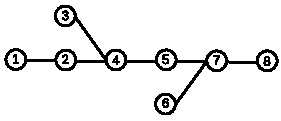
\includegraphics[width=0.8\textwidth]{ex-struct-process-2}}

\vspace{15pt}

Dove:
\begin{enumerate}[label=$F_{\arabic*}$:]
    \item fase di stesura della pasta;
    \item fase di aggiunta della pasta al piatto;
    \item fase di produzione del sugo di pomodoro;
    \item fase di aggiunta del pomodoro lavorato (sugo);
    \item fase di aggiunta della mozzarella;
    \item fase di taglio del prosciutto in fette;
    \item fase di aggiunta del prosciutto lavorato (fette di prosciutto);
    \item fase di cottura.
\end{enumerate}
\begingroup\itshape\fontsize{10pt}{10pt}\selectfont
    Si noti che con tale struttura ci sono più modi per rappresentare lo stesso procedimento
    di preparazione di un piatto: ad esempio si potrebbe scambiare $F_{1}$ con $F_{2}$ senza
    cambiare il \textnormal{senso} del procedimento; oppure si potrebbe spostare la fase $F_{7}$ a
    prima della fase $F_{6}$ e inserire una nuova fase al posto vuoto lasciato da $F_{7}$ che
    indica di mettere insieme i due \textnormal{semilavorati} (la pizza col pomodoro e la mozzarella
    e le fette di prosciutto).
\endgroup
\vspace{10pt}

Facciamo l'ipotesi che il cliente voglia come variazione la rimozione del pomodoro
(pizza bianca). In tal caso devono essere rimosse due fasi (anche se la variazione è
una sola!): $F_{3}$ e $F_{4}$. Se invece quello precedente fosse stato il procedimento
di una pizza margherita e il cliente avesse indicato come variazione l'aggiunta del
prosciutto, si sarebbero dovute aggiungere due fasi: $F_{6}$ e $F_{7}$.

Questo dimostra che è necessario che ogni variazione possa effettuare anche più di un'operazione
elementare (aggiunta o rimozione) sul procedimento strutturato.

L'entità {\tt ModificaFase} (con le sue entità figlie) è stata aggiunta al {\it diagramma
entità-relazione} (disponibile \vpageref{diagram.1}) allo scopo di permettere
ad ogni variazione di {\it modificare} anche più fasi: ogni variazione ha più
{\tt ModificaFase} e ogni {\tt ModificaFase} rappresenta la modifica (aggiunta, eliminazione, sostituzione)
di una e una sola fase (la sostituzione coinvolge però due fasi: quella da togliere e quella da aggiungere).

Le fasi che fanno parte di variazioni (come le fasi $F_{6}$ e $F_{7}$ nel caso del procedimento
della pizza margherita) non vengono confuse dal database con le fasi della ricetta {\it normale}:
infatti le fasi che fanno parte di variazioni si troveranno come {\it chiavi esterne}
all'interno dell'entità {\tt AggiuntaFase} (o {\tt SostituzioneFase}) per mezzo della relazione
{\tt Nuova}, e quindi il database saprà distinguerle da quelle della ricetta normale
(vedere il diagramma \vpageref{diagram.1}).

